% Options for packages loaded elsewhere
\PassOptionsToPackage{unicode}{hyperref}
\PassOptionsToPackage{hyphens}{url}
%
\documentclass[
]{article}
\usepackage{lmodern}
\usepackage{amssymb,amsmath}
\usepackage{ifxetex,ifluatex}
\ifnum 0\ifxetex 1\fi\ifluatex 1\fi=0 % if pdftex
  \usepackage[T1]{fontenc}
  \usepackage[utf8]{inputenc}
  \usepackage{textcomp} % provide euro and other symbols
\else % if luatex or xetex
  \usepackage{unicode-math}
  \defaultfontfeatures{Scale=MatchLowercase}
  \defaultfontfeatures[\rmfamily]{Ligatures=TeX,Scale=1}
\fi
% Use upquote if available, for straight quotes in verbatim environments
\IfFileExists{upquote.sty}{\usepackage{upquote}}{}
\IfFileExists{microtype.sty}{% use microtype if available
  \usepackage[]{microtype}
  \UseMicrotypeSet[protrusion]{basicmath} % disable protrusion for tt fonts
}{}
\makeatletter
\@ifundefined{KOMAClassName}{% if non-KOMA class
  \IfFileExists{parskip.sty}{%
    \usepackage{parskip}
  }{% else
    \setlength{\parindent}{0pt}
    \setlength{\parskip}{6pt plus 2pt minus 1pt}}
}{% if KOMA class
  \KOMAoptions{parskip=half}}
\makeatother
\usepackage{xcolor}
\IfFileExists{xurl.sty}{\usepackage{xurl}}{} % add URL line breaks if available
\IfFileExists{bookmark.sty}{\usepackage{bookmark}}{\usepackage{hyperref}}
\hypersetup{
  hidelinks,
  pdfcreator={LaTeX via pandoc}}
\urlstyle{same} % disable monospaced font for URLs
\usepackage[left=1cm,right=1cm,top=2cm,bottom=2cm]{geometry}
\usepackage{graphicx,grffile}
\makeatletter
\def\maxwidth{\ifdim\Gin@nat@width>\linewidth\linewidth\else\Gin@nat@width\fi}
\def\maxheight{\ifdim\Gin@nat@height>\textheight\textheight\else\Gin@nat@height\fi}
\makeatother
% Scale images if necessary, so that they will not overflow the page
% margins by default, and it is still possible to overwrite the defaults
% using explicit options in \includegraphics[width, height, ...]{}
\setkeys{Gin}{width=\maxwidth,height=\maxheight,keepaspectratio}
% Set default figure placement to htbp
\makeatletter
\def\fps@figure{htbp}
\makeatother
\setlength{\emergencystretch}{3em} % prevent overfull lines
\providecommand{\tightlist}{%
  \setlength{\itemsep}{0pt}\setlength{\parskip}{0pt}}
\setcounter{secnumdepth}{-\maxdimen} % remove section numbering
\usepackage{fancyhdr} \pagestyle{fancy} \usepackage{graphicx} \usepackage{eurosym} \usepackage{xcolor} \usepackage{booktabs,xcolor} \definecolor{myblue}{HTML}{5F7ED9} \definecolor{wblight}{HTML}{f8f4fc} \rhead{
\includegraphics[width=3.5cm]{gender-logo.png}} \lhead{
\includegraphics[width=1.25cm]{Flag_of_Colombia.png}\fontsize{22}{1}\selectfont\textbf{ COLOMBIA \textcolor{myblue}{GENDER LANDSCAPE}}} \rfoot{Last compiled on 07 April, 2022} \lfoot{
\includegraphics[width=19.5cm]{footer.png}} \fancypagestyle{plain}{\pagestyle{fancy}} \pagenumbering{gobble} \usepackage[defaultfam,tabular,lining]{montserrat} \usepackage[fontsize=8pt]{scrextend} \usepackage{float} \restylefloat{table} \usepackage{multicol} \newcommand{\hideFromPandoc}[1]{#1} \hideFromPandoc{ \let\Begin\begin \let\End\end } \usepackage{caption} \captionsetup{skip=0pt} \setlength{\headsep}{1.1cm}
\usepackage{booktabs}
\usepackage{longtable}
\usepackage{array}
\usepackage{multirow}
\usepackage{wrapfig}
\usepackage{float}
\usepackage{colortbl}
\usepackage{pdflscape}
\usepackage{tabu}
\usepackage{threeparttable}
\usepackage{threeparttablex}
\usepackage[normalem]{ulem}
\usepackage{makecell}
\usepackage{xcolor}

\author{}
\date{\vspace{-2.5em}}

\begin{document}

\begin{wraptable}{r}{0pt}\begingroup\fontsize{8}{10}\selectfont

\begin{tabular}[t]{lll}

\textbf{Comparison} & \textbf{Baseline} & \textbf{Region}\\
\midrule
Higher Performance & 
\includegraphics[width=0.1in, height=0.1in]{upicon.png} & \cellcolor[HTML]{46F884}{}\\
Equal/No Change & 
\includegraphics[width=0.1in, height=0.1in]{righticon.png} & \cellcolor[HTML]{E1DD37}{}\\
Lower Performance & 
\includegraphics[width=0.1in, height=0.1in]{downicon.png} & \cellcolor[HTML]{F05B12}{}\\
No Data & 
\includegraphics[width=0.1in, height=0.1in]{naicon.png} & \cellcolor{lightgray}{}\\

\end{tabular}
\endgroup{}\end{wraptable}
\fontsize{9}{8}\selectfont

This brief provides a quick overview of the gender landscape in Colombia
on some key indicators. For Colombia, the highest performing indicators
relative to the baseline year are Firms with female top manager (\% of
firms) and Proportion of seats held by women in national parliaments
(\%). The largest declines relative to the baseline year are Prevalence
of current tobacco use and Adolescent fertility rate (births per 1,000
women ages 15-19). \normalsize \vspace{2pt}

\renewcommand{\arraystretch}{1.15}

\begingroup\fontsize{8}{10}\selectfont

\begin{ThreePartTable}
\begin{TableNotes}[para]
\item \textit{Note: } 
\item Data retrieved from World Bank Gender Data Portal. Country Baseline provides a reference point for the indicator, circa 2010. LAC = Includes the 42 countries (all income levels) in Latin America and the Caribbean, as classified by The World Bank Group. UMC = In FY21, upper- middle-income countries are those with a GNI per capita between \$4,046 and \$12,535 (calculated using the World Bank Atlas method).
\end{TableNotes}
\begin{longtable}[t]{>{\raggedright\arraybackslash}p{9cm}>{\raggedright\arraybackslash}p{.85cm}>{\raggedleft\arraybackslash}p{.85cm}>{\raggedleft\arraybackslash}p{.85cm}>{}r>{}r>{\raggedleft\arraybackslash}p{.85cm}>{\raggedleft\arraybackslash}p{.85cm}>{\raggedleft\arraybackslash}p{.85cm}}
\toprule
\multicolumn{2}{c}{ } & \multicolumn{4}{c}{Columbia's Performance} & \multicolumn{3}{c}{Peers Comparison} \\
\cmidrule(l{3pt}r{3pt}){3-6} \cmidrule(l{3pt}r{3pt}){7-9}
Measure & Gender & Baseline & Year & Rating & Year  & Region & Income & Global\\
\midrule
\endfirsthead
\multicolumn{9}{@{}l}{\textit{(continued)}}\\
\toprule
Measure & Gender & Baseline & Year & Rating & Year  & Region & Income & Global\\
\midrule
\endhead

\endfoot
\bottomrule
\insertTableNotes
\endlastfoot
\addlinespace[0.3em]
\multicolumn{9}{l}{\cellcolor{lightgray}{\textbf{HUMAN ENDOWMENTS}}}\\
\hline
 & Female & 8.1 & 2010 & \cellcolor{lightgray}{\textcolor{black}{\textbf{8.6}}} & 2020
\includegraphics[width=0.1in, height=0.1in]{righticon.png} & NA & NA & NA\\
\nopagebreak
\multirow{-2}{9cm}{\raggedright\arraybackslash \href{http://graphicacy-wb-gender-portal.s3-website-us-east-1.amazonaws.com/indicators/hd-hci-lays/}{Learning-Adjusted Years of School}} & Male & 8.3 & 2010 & \cellcolor{lightgray}{\textcolor{black}{\textbf{8.6}}} & 2020
\includegraphics[width=0.1in, height=0.1in]{righticon.png} & NA & NA & NA\\
\cmidrule{1-9}\pagebreak[0]
 & Female & 404.3 & 2010 & \cellcolor{lightgray}{\textcolor{black}{\textbf{415.3}}} & 2020
\includegraphics[width=0.1in, height=0.1in]{righticon.png} & NA & NA & NA\\
\nopagebreak
\multirow{-2}{9cm}{\raggedright\arraybackslash \href{http://graphicacy-wb-gender-portal.s3-website-us-east-1.amazonaws.com/indicators/hd-hci-hlos}{Harmonized Test Scores}} & Male & 419.9 & 2010 & \cellcolor{lightgray}{\textcolor{black}{\textbf{423.0}}} & 2020
\includegraphics[width=0.1in, height=0.1in]{righticon.png} & NA & NA & NA\\
\cmidrule{1-9}\pagebreak[0]
 & Female & 41.3 & 2010 & \cellcolor[HTML]{E1DD37}{\textcolor{black}{\textbf{59.0}}} & 2019
\includegraphics[width=0.1in, height=0.1in]{upicon.png} & 61.7 & 63.0 & 43.2\\
\nopagebreak
\multirow{-2}{9cm}{\raggedright\arraybackslash \href{http://graphicacy-wb-gender-portal.s3-website-us-east-1.amazonaws.com/indicators/se-ter-enrr/}{School enrollment, tertiary}} & Male & 37.5 & 2010 & \cellcolor[HTML]{E1DD37}{\textcolor{black}{\textbf{51.1}}} & 2019
\includegraphics[width=0.1in, height=0.1in]{upicon.png} & 46.8 & 52.6 & 37.5\\
\cmidrule{1-9}\pagebreak[0]
\href{http://graphicacy-wb-gender-portal.s3-website-us-east-1.amazonaws.com/indicators/se-ter-grad-fe-zs/}{Female share of graduates from STEM programmes, tertiary (\%)} &  & 36.8 & 2002 & \cellcolor{lightgray}{\textcolor{black}{\textbf{33.4}}} & 2018
\includegraphics[width=0.1in, height=0.1in]{downicon.png} & NA & NA & NA\\
\cmidrule{1-9}\pagebreak[0]
\href{http://graphicacy-wb-gender-portal.s3-website-us-east-1.amazonaws.com/indicators/sp-dyn-tfrt-in/}{Fertility rate, total (births per woman)} &  & 2.0 & 2010 & \cellcolor[HTML]{46F884}{\textcolor{black}{\textbf{1.8}}} & 2019
\includegraphics[width=0.1in, height=0.1in]{downicon.png} & 2.0 & 1.8 & 2.4\\
\cmidrule{1-9}\pagebreak[0]
\href{http://graphicacy-wb-gender-portal.s3-website-us-east-1.amazonaws.com/indicators/sh-sta-mmrt/}{Maternal mortality ratio (per 100,000 live births)} &  & 85.0 & 2010 & \cellcolor[HTML]{F05B12}{\textcolor{black}{\textbf{83.0}}} & 2017
\includegraphics[width=0.1in, height=0.1in]{righticon.png} & 74.0 & 41.0 & 211.0\\
\cmidrule{1-9}\pagebreak[0]
 & Female & 5.8 & 2010 & \cellcolor[HTML]{46F884}{\textcolor{black}{\textbf{3.7}}} & 2018
\includegraphics[width=0.1in, height=0.1in]{downicon.png} & 10.1 & 5.6 & 9.3\\
\nopagebreak
\multirow{-2}{9cm}{\raggedright\arraybackslash \href{http://graphicacy-wb-gender-portal.s3-website-us-east-1.amazonaws.com/indicators/sh-prv-smok}{Prevalence of current tobacco use}} & Male & 16.2 & 2010 & \cellcolor[HTML]{46F884}{\textcolor{black}{\textbf{12.2}}} & 2018
\includegraphics[width=0.1in, height=0.1in]{downicon.png} & 21.7 & 41.4 & 38.5\\
\cmidrule{1-9}\pagebreak[0]
\addlinespace[0.3em]
\multicolumn{9}{l}{\cellcolor{lightgray}{\textbf{ECONOMIC OPPORTUNITY}}}\\
\hline
 & Female & 55.4 & 2010 & \cellcolor[HTML]{E1DD37}{\textcolor{black}{\textbf{50.3}}} & 2020
\includegraphics[width=0.1in, height=0.1in]{downicon.png} & 46.1 & 55.1 & 45.9\\
\nopagebreak
\multirow{-2}{9cm}{\raggedright\arraybackslash \href{http://graphicacy-wb-gender-portal.s3-website-us-east-1.amazonaws.com/indicators/sl-tlf-acti-zs/}{Labor force participation rate}} & Male & 81.0 & 2010 & \cellcolor[HTML]{E1DD37}{\textcolor{black}{\textbf{75.9}}} & 2020
\includegraphics[width=0.1in, height=0.1in]{righticon.png} & 70.1 & 72.4 & 71.3\\
\cmidrule{1-9}\pagebreak[0]
 & Female & 49.1 & 2010 & \cellcolor[HTML]{F05B12}{\textcolor{black}{\textbf{46.1}}} & 2019
\includegraphics[width=0.1in, height=0.1in]{righticon.png} & 33.8 & 38.3 & 44.0\\
\nopagebreak
\multirow{-2}{9cm}{\raggedright\arraybackslash \href{http://graphicacy-wb-gender-portal.s3-website-us-east-1.amazonaws.com/indicators/sl-emp-vuln-zs/}{Vulnerable employment}} & Male & 47.7 & 2010 & \cellcolor[HTML]{F05B12}{\textcolor{black}{\textbf{45.8}}} & 2019
\includegraphics[width=0.1in, height=0.1in]{righticon.png} & 33.4 & 35.6 & 43.4\\
\cmidrule{1-9}\pagebreak[0]
 & Female & 32.8 & 2010 & \cellcolor[HTML]{E1DD37}{\textcolor{black}{\textbf{32.4}}} & 2019
\includegraphics[width=0.1in, height=0.1in]{righticon.png} & 29.5 & NA & NA\\
\nopagebreak
\multirow{-2}{9cm}{\raggedright\arraybackslash \href{http://graphicacy-wb-gender-portal.s3-website-us-east-1.amazonaws.com/indicators/sl-uem-neet-zs/}{Share of youth not in education, employment or training}} & Male & 14.4 & 2010 & \cellcolor[HTML]{46F884}{\textcolor{black}{\textbf{15.6}}} & 2019
\includegraphics[width=0.1in, height=0.1in]{righticon.png} & 18.3 & NA & NA\\
\cmidrule{1-9}\pagebreak[0]
 & Female & 7.0 & 2010 & \cellcolor[HTML]{E1DD37}{\textcolor{black}{\textbf{6.6}}} & 2019
\includegraphics[width=0.1in, height=0.1in]{righticon.png} & 7.1 & 17.8 & 25.3\\
\nopagebreak
\multirow{-2}{9cm}{\raggedright\arraybackslash \href{http://graphicacy-wb-gender-portal.s3-website-us-east-1.amazonaws.com/indicators/se-ter-grad-fe-zs}{Employment in agriculture}} & Male & 26.2 & 2010 & \cellcolor[HTML]{F05B12}{\textcolor{black}{\textbf{22.3}}} & 2019
\includegraphics[width=0.1in, height=0.1in]{downicon.png} & 18.0 & 23.5 & 27.6\\
\cmidrule{1-9}\pagebreak[0]
 & Female & NA & NA & \cellcolor{lightgray}{\textcolor{black}{\textbf{5.0}}} & 2017
\includegraphics[width=0.1in, height=0.1in]{naicon.png} & NA & NA & NA\\
\nopagebreak
\multirow{-2}{9cm}{\raggedright\arraybackslash \href{http://graphicacy-wb-gender-portal.s3-website-us-east-1.amazonaws.com/indicators/sg-tim-uwrk/}{Proportion of time spent on unpaid domestic and care work}} & Male & NA & NA & \cellcolor{lightgray}{\textcolor{black}{\textbf{2.9}}} & 2017
\includegraphics[width=0.1in, height=0.1in]{naicon.png} & NA & NA & NA\\
\cmidrule{1-9}\pagebreak[0]
\href{http://graphicacy-wb-gender-portal.s3-website-us-east-1.amazonaws.com/indicators/ic-wef-llco-zs/}{Share of female business owners (\% of total business owners)} &  & NA & NA & \cellcolor{lightgray}{\textcolor{black}{\textbf{NA}}} & NA
\includegraphics[width=0.1in, height=0.1in]{naicon.png} & NA & NA & NA\\
\cmidrule{1-9}\pagebreak[0]
\href{http://graphicacy-wb-gender-portal.s3-website-us-east-1.amazonaws.com/indicators/ic-wef-llco-zs/}{Share of male business owners  (\% of total business owners)} &  & NA & NA & \cellcolor{lightgray}{\textcolor{black}{\textbf{NA}}} & NA
\includegraphics[width=0.1in, height=0.1in]{naicon.png} & NA & NA & NA\\
\cmidrule{1-9}\pagebreak[0]
 & Female & NA & NA & \cellcolor[HTML]{F05B12}{\textcolor{black}{\textbf{42.5}}} & 2017
\includegraphics[width=0.1in, height=0.1in]{naicon.png} & 52.0 & 69.3 & 64.8\\
\nopagebreak
\multirow{-2}{9cm}{\raggedright\arraybackslash \href{http://graphicacy-wb-gender-portal.s3-website-us-east-1.amazonaws.com/indicators/fin1-t-a/}{Account ownership at a financial institution or with a mobile-money-service provider}} & Male & NA & NA & \cellcolor[HTML]{F05B12}{\textcolor{black}{\textbf{49.4}}} & 2017
\includegraphics[width=0.1in, height=0.1in]{naicon.png} & 58.6 & 77.0 & 72.3\\
\cmidrule{1-9}\pagebreak[0]
\addlinespace[0.3em]
\multicolumn{9}{l}{\cellcolor{lightgray}{\textbf{VOICE AND AGENCY}}}\\
\hline
\href{http://graphicacy-wb-gender-portal.s3-website-us-east-1.amazonaws.com/indicators/sp-2024-fe-zs/}{Women who were first married by age 18 (\% of women ages 20-24)} &  & 23.0 & 2010 & \cellcolor{lightgray}{\textcolor{black}{\textbf{23.4}}} & 2015
\includegraphics[width=0.1in, height=0.1in]{righticon.png} & NA & NA & NA\\
\cmidrule{1-9}\pagebreak[0]
\href{http://graphicacy-wb-gender-portal.s3-website-us-east-1.amazonaws.com/indicators/sp-ado-tfrt/}{Adolescent fertility rate (births per 1,000 women ages 15-19)} &  & 76.8 & 2010 & \cellcolor[HTML]{E1DD37}{\textcolor{black}{\textbf{64.3}}} & 2019
\includegraphics[width=0.1in, height=0.1in]{downicon.png} & 61.2 & 29.5 & 41.5\\
\cmidrule{1-9}\pagebreak[0]
\href{http://graphicacy-wb-gender-portal.s3-website-us-east-1.amazonaws.com/indicators/sg-gen-parl-zs/}{Proportion of seats held by women in national parliaments (\%)} &  & 12.7 & 2010 & \cellcolor[HTML]{F05B12}{\textcolor{black}{\textbf{18.3}}} & 2020
\includegraphics[width=0.1in, height=0.1in]{upicon.png} & 32.8 & 26.5 & 25.6\\
\cmidrule{1-9}\pagebreak[0]
\href{http://graphicacy-wb-gender-portal.s3-website-us-east-1.amazonaws.com/indicators/ic-frm-femm-zs/}{Firms with female top manager (\% of firms)} &  & 12.1 & 2010 & \cellcolor[HTML]{E1DD37}{\textcolor{black}{\textbf{18.9}}} & 2017
\includegraphics[width=0.1in, height=0.1in]{upicon.png} & 20.1 & 19.1 & 17.8\\
\cmidrule{1-9}\pagebreak[0]
\href{http://graphicacy-wb-gender-portal.s3-website-us-east-1.amazonaws.com/indicators/sg-vaw-1549-zs/}{Proportion of women subjected to physical and/or sexual violence in the last 12 months (\% of women age 15-49)} &  & NA & NA & \cellcolor{lightgray}{\textcolor{black}{\textbf{18.4}}} & 2015
\includegraphics[width=0.1in, height=0.1in]{naicon.png} & NA & NA & NA\\
\cmidrule{1-9}\pagebreak[0]
 & Female & NA & NA & \cellcolor{lightgray}{\textcolor{black}{\textbf{9.1}}} & 2017
\includegraphics[width=0.1in, height=0.1in]{naicon.png} & NA & 36.1 & 27.7\\
\nopagebreak
\multirow{-2}{9cm}{\raggedright\arraybackslash \href{http://graphicacy-wb-gender-portal.s3-website-us-east-1.amazonaws.com/indicators/fin14abca-t-d/}{Used the internet to pay bills or to buy something online in the past year}} & Male & NA & NA & \cellcolor{lightgray}{\textcolor{black}{\textbf{14.5}}} & 2017
\includegraphics[width=0.1in, height=0.1in]{naicon.png} & NA & 39.0 & 30.3\\*
\end{longtable}
\end{ThreePartTable}
\endgroup{}

\newpage
\clearpage

\fontsize{14}{8}\selectfont

Gender Equality in Colombia \normalsize

\fboxrule.6pt\fboxsep6pt \fcolorbox{myblue}{wblight}{\color{black}
\begin{minipage}[c][2.5cm][t]{3.45cm}
\raggedright\fontsize{12}{1}\selectfont   
\textbf{One in four} 
\normalsize
  
\vspace{.3cm}
  
\emph{women were first married by age 18}
\end{minipage}} \fcolorbox{myblue}{wblight}{\color{black}
\begin{minipage}[c][2.5cm][t]{3.45cm}
\raggedright\fontsize{12}{1}\selectfont   
\textbf{Two in five} 
\normalsize
  
\vspace{.3cm}
 
\emph{women hold an account at a financial institution}
\end{minipage}} \fcolorbox{myblue}{wblight}{\color{black}
\begin{minipage}[c][2.5cm][t]{3.45cm}
\raggedright\fontsize{12}{1}\selectfont   
\textbf{64} 
\normalsize
  
\vspace{.3cm}
 
\emph{young women gave birth as adolescents per 1000 women}
\end{minipage}} \fcolorbox{myblue}{wblight}{\color{black}
\begin{minipage}[c][2.5cm][t]{3.45cm}
\raggedright\fontsize{12}{1}\selectfont   
\textbf{One in five} 
\normalsize
  
\vspace{.3cm}
 
\emph{firms have a female top manager}
\end{minipage}} \fcolorbox{myblue}{wblight}{\color{black}
\begin{minipage}[c][2.5cm][t]{3.45cm}
\raggedright\fontsize{12}{1}\selectfont   
\textbf{One in five} 
\normalsize
  
\vspace{.3cm}
 
\emph{seats in national parliament are held by women}
\end{minipage}} \vspace{.2cm}

\fontsize{14}{8}\selectfont

Gender Equality and the Law \normalsize

Women, Business and the Law 2021 presents an index covering 190
economies and structured around the life cycle of a working woman. In
total, 35 questions are scored across the eight indicators. Colombia
scores 81.9 out of 100, higher than the regional average observed across
Latin America \& Caribbean (80.1).

\begin{center}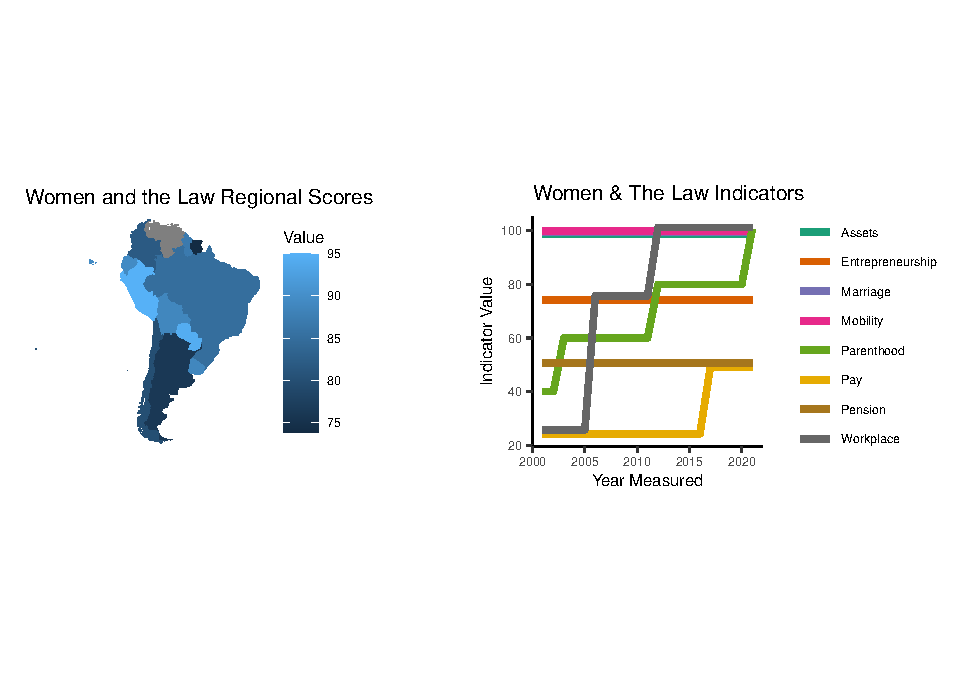
\includegraphics[width=1\linewidth,trim={0 3.1cm 0 3.1cm},clip]{Gender-Briefs_files/figure-latex/genderlaw-1} \end{center}

\begin{center}\rule{0.5\linewidth}{0.5pt}\end{center}

\fontsize{14}{8}\selectfont

Curated resources to address gender gaps \normalsize

Click on the links below for more information

\begin{wraptable}{l}{0pt}\begingroup\fontsize{8}{10}\selectfont

\begin{tabular}[t]{>{\raggedright\arraybackslash}p{9cm}>{\raggedright\arraybackslash}p{9cm}}
\toprule
\begingroup\fontsize{10}{12}\selectfont \textbf{Global Resources}\endgroup & \begingroup\fontsize{10}{12}\selectfont \textbf{Regional Resources}\endgroup\\
\midrule
\addlinespace[0.3em]
\multicolumn{2}{c}{\textbf{Human Endowments}}\\
\href{https://openknowledge.worldbank.org/handle/10986/34317}{The Equality Equation: Advancing the Participation of Women and Girls in STEM} & \href{https://worldbankgroup.sharepoint.com/sites/LCR/Documents/Gender/Country%20Scorecards/Facilitating%20the%20School%20to%20Work%20Transition%20of%20Young%20Women.pdf}{Facilitating school-to-work transitions}\\
\href{https://documents.worldbank.org/en/publication/documents-reports/documentdetail/530891498511398503/economic-impacts-of-child-marriage-global-synthesis-report}{Economic impacts of child marriage: global synthesis report} & \href{https://worldbankgroup.sharepoint.com/sites/LCR/Documents/Gender/Country%20Scorecards/Atracting%20more%20Young%20Women%20into%20STEM%20Fields.pdf}{Attracting more women into STEM felds}\\
\href{}{} & \href{https://worldbankgroup.sharepoint.com/sites/LCR/Documents/Gender/Country%20Scorecards/Reducing%20Boys'%20School%20Droppout%20and%20Helping%20Boys%20at%20Risk.pdf}{Reducing boys’ school dropout and helping boys at risk}\\
\addlinespace[0.3em]
\multicolumn{2}{c}{\textbf{Economic Opportunity}}\\
\href{https://documents.worldbank.org/en/publication/documents-reports/documentdetail/450971635788989068/childcare-and-mothers-labor-market-outcomes-in-lower-and-middle-income-countries}{Childcare and Mothers’ Labor Market Outcomes in Lower- and Middle-Income Countries} & \href{https://worldbankgroup.sharepoint.com/sites/LCR/Documents/Gender/Country%20Scorecards/Expanding%20Access%20to%20Affordable%20and%20Quality%20Care.pdf}{Expanding access to affordable and quality care}\\
\href{https://openknowledge.worldbank.org/handle/10986/36940}{Breaking Barriers: Female Entrepreneurs Who Cross Over to Male-Dominated Sectors} & \href{https://worldbankgroup.sharepoint.com/sites/LCR/Documents/Gender/Country%20Scorecards/Improving%20Women's%20Access%20to%20Quality%20Employment.pdf}{Improving women’s access to quality employment}\\
\href{https://openknowledge.worldbank.org/handle/10986/36257}{Measuring Women and Men’s Work: Main Findings from a Joint ILO and World Bank Study in Sri Lanka} & \href{https://worldbankgroup.sharepoint.com/sites/LCR/Documents/Gender/Country%20Scorecards/Improving%20the%20Performance%20of%20Women-Owned%20Firms.pdf}{Improving the performance of women-owned firms}\\
\href{}{} & \href{https://worldbankgroup.sharepoint.com/sites/LCR/Documents/Gender/Country%20Scorecards/Improving%20the%20Performance%20of%20Women-Owned%20Firms.pdf}{Increasing women’s ownership and control of productive assets}\\
\addlinespace[0.3em]
\multicolumn{2}{c}{\textbf{Voice and Agency}}\\
\href{https://www.whatworks.co.za/documents/publications/374-evidence-reviewfweb/file}{What Works to Prevent Violence against Women} & \href{https://worldbankgroup.sharepoint.com/sites/LCR/Documents/Gender/Country%20Scorecards/Preventing%20and%20Addressing%20Violence%20Against%20Women%20and%20Girls.pdf}{Preventing and addressing violence against women and girls}\\
\href{}{} & \href{https://worldbankgroup.sharepoint.com/sites/LCR/Documents/Gender/Country%20Scorecards/Reducing%20Teen%20Pregnancy.pdf}{Reducing teen pregnancy}\\
\addlinespace[0.3em]
\multicolumn{2}{c}{\textbf{Girls Green, Resilient, \& Economic Development}}\\
\href{https://openknowledge.worldbank.org/handle/10986/35202}{Gender Dimensions of Disaster Risk and Resilience: Existing Evidence} & \href{}{}\\
\href{https://documents.worldbank.org/en/publication/documents-reports/documentdetail/895601643214591612/the-gender-dimensions-of-forced-displacement-a-synthesis-of-new-research}{The Gender Dimensions of Forced Displacement: A Synthesis of New Research} & \href{}{}\\
\bottomrule
\end{tabular}
\endgroup{}\end{wraptable}

\end{document}
